\section{Notes form meeting at 2AUG22}
\label{sec:meetingNotes}
There are two different models to consider: (1) the ``IBC" model, and (2) the ``simple" model.

% IBC
In the IBC model \cite{IBC} (which might be the initial intention of \hc), accounts from different subnets can communicate with each other using bridges. This allows two accounts to perform cross subnet interactions directly using the 
IBC protocol, which in \hc s case will be the cross-net message transfer mechanism.\guy{I need to better understand \cite{IBC} to be sure, but it appears that interaction between two accounts from different subnets requires not only trust between the accounts but also that \emph{the two subnets trust each other}.}

% simple model
In the simple model (which is described in this document), accounts cannot communicate directly with other subnets, in general. Rather, their cross-net interactions are limited to basic operations between parent and child accounts. In particular, to token transfers between accounts of the same user. Moreover, in order for a user $u_i$ to interact with a user $u_j$ they must both have accounts on a shared subnet.\\

Besides the need for a more complex mechanism to support cross-net messages in the ``IBC" approach, the main difference comes from what is the offered tradeoff.
Essentially, in ``IBC", the scalability comes on the expense of trust, while in the ``simple" approach the scalability comes from locality, and is therefore limited by its existence.
In particular, IBC requires stronger trust assumptions (a user needs to trust all subnets in the path of a cross-net interaction), but does not need to maintain a hierarchy of accounts, while ``simple" only requires that a user trusts the common ancestor subnet, but also requires to have an account in the common ancestor.\\
%
\red{Q: How much benefits can be drawn from the ``simple" model (in terms of scalability)?}\\
\red{Q: How limiting is the stronger trust requirements on the usage of the IBC model?}\\
\red{Q: Can IBC be implemented independently as a ``shortcut" between subnets in the ``simple" model?}


\subsection{Additional points}
\begin{itemize}
    \item It might be that batching is the main benefit of implementing IBC via \hc. In that case, we should consider whether this can be treated orthogonally (e.g., via a dedicated smart contract), rather than entangling it with \hc. On the other hand, maybe the entanglement provides implementation benefits, e.g., speedup. \arp{probs in same smart contract but imo added feature: not necessary to spawn a subnet. 'Simple' -> base functionality, IBC -> optional added features}
    \item It appears that currently the system requires a single ``almighty" token to support the IBC implementation (which is sufficient for MVP). Using the simple approach, naturally supports internal token generation. The only requirement is that the balances of $\SN$ in \parent{$\SN$} are in a token that is supported in \parent{$\SN$}.
\end{itemize}

%%%%%%%%%%%%%%%%%%%%%%%%%%%%%%%%%%%%%%%%%%%%%%%%%%%%%%
%%%%%%%%%%%%%%%%%%%%%%%%%%%%%%%%%%%%%%%%%%%%%%%%%%%%%%
\section{Meeting Notes from Vaduz}

Money / coins / tokens can only be sent from a concrete account at the parent to a concrete account on the subnet

SA: Subnet actor (smart contract) on the parent, holding all information relevant for a single subnet.
$G$: Guy's account on the parent
$g$: Guy's account on the subnet
$g'$: Guy's subnet balance as seen by the parent, represented as an entry in the SA's account balances.

\paragraph{State of the smart contract contains:}
\begin{itemize}
    \item Account balances for all the children accounts in the subnet.
    \item A governance account and an associated policy how this account is funded and under which conditions money is transferred from it.
        The purpose of a governance account is to store funds associated with running the subnet (the subnet's "commons"). E.g., the transaction fees incurred by submitting checkpoints might be reimbursed from the governance account (under conditions specified by some policy). It can be funded, for example, by transaction fees within the subnet. The governance account might be involved in providing incentives for child validators to participate (rewards) and / or to behave correctly (slashing). The governance account has a corresponding account in the child subnet as well. It can be funded, e.g., through withdrawals from the child subnet.
    \item Validators' set + metadata (e.g. voting rights/collateral/stake/...)
    \begin{itemize}
        \item Consensus protocol
        \item Subnet configuration (probably a pointer to the data)
        \item Governance rules
    \end{itemize}
    \item A function $checkProofOfGlobalFinality(localState, proof)\rightarrow bool$. This function defines what constitutes a proof of global finality of a state of the child.
        E.g., this could be a set of signatures of subnet validators. For a longest-chain-based subnet, the definition of this function would involve a depth parameter, such that all blocks deeper than depth are considered final. If a reorganization of the child happens deeper than that depth, it can be considered as a failure of the whole subnet.
    \item Slashing functionality \arp{and checkpointing rules}
\end{itemize}

\paragraph{Interactions between parent and child}
It is likely that in practice, for efficiency reasons, multiple interactions will be batched together (possibly even combining withdrawals, deposits and checkpoint into a single transaction).
Nevertheless, we present here a cleaner version where operations are handled independently as it trivially generalizes to the batched version.
\begin{itemize}
    \item \textbf{DEPOSIT money (e.g. 2 coins) (transfer from G to g).}
    \begin{itemize}
        \item $\langle TX(G \rightarrow^{+2} SA:g')\rangle_{Guy}$: Transaction sending 2 coins from G to $SA:g'$, signed by Guy.
        \item Observer(s) of parent state create a TX for the child: $TX(g+2, proof)$ that adds 2 to g (when accepted as valid). The validity of this transaction must only depend on the transactions preceding it and itself.
        Example options for checking the validity of $TX(g+2, proof)$:
        \begin{enumerate}
            \item \textbf{on-chain voting}:
            When locally observing the parent state change, each subnet validator submits $\langle TX(g+2)\rangle_{Validator}$ to the child SMR system.
            When a quorum (e.g. $f+1$) such transactions signed by different validators are ordered, the last of them has the effect of increasing $g$ by 2.
            \item \textbf{off-chain voting}:
            Like on-chain voting, but all the transactions (signed by different validators) are gathered off-band and submitted (by any client to the child SMR system) as a single transaction $TX(g+2, proof)$, where the $proof$ consists of a quorum of child subnet validators' signatures.
            \item \textbf{local validity check} (simpler, efficient, \textit{weaker guarantees}): $proof$ contains a pointer to the block containing $\langle TX(G \rightarrow^{+2} SA:g')\rangle_{Guy}$ at the parent, together with the height~$h$ of that block.
            To validate the $TX$ the child queries the parent about $TX$, if it exists -- return valid, else -- return invalid. If invalid but the parent is still below height~$h$, then query again when parent reaches height~$h$.
            \item \textbf{subnet protocol integration}: Using PBFT as an example. Any client of the child subnet submits $TX(g+2)$ to the child (one is enough). On reception of a PBFT Preprepare message, a validator only sends the Prepare message once it observes the corresponding parent state change. This way, the child subnet's validators implicitly vote on the validity of $TX(g+2)$. Once it is committed, it is considered valid by all validators, even those that did not vote for it.
        \end{enumerate}
    \end{itemize}
    
    \item \textbf{WITHDRAW money (e.g. 2 coins) (transfer from g to G)}
    \begin{itemize}
        \item $\langle TX(g-2)\rangle_{Guy}$ (transaction ``burning" 2 coins from $g$, signed by Guy) on the child.
        \item Observer(s) of child state create a TX for the parent:  $\langle TX(SA:g' \rightarrow^{+2} G, proof)\rangle_{Guy}$ that decreases SA:g' by 2 and adds 2 to G (when accepted as valid). Validating this transaction must only depend on $proof$ and $SA$s internal state (which is visible at the parent).
        Example options for checking the validity of $\langle TX(SA:g' \rightarrow^{+2} G, proof)\rangle_{Guy}$:
        \begin{enumerate}
            \item \textbf{Threshold signature from the child subnet validators}:\footnote{An example is an $f+1$ threshold signature.}
            $proof$ contains a threshold signature from the child validators (which are listed in $SA$). A partial signature (for the threshold) from a validator~$v$ affirms that~$v$ considers $\langle TX(g-2)\rangle_{Guy}$ as stable in the child subnet.
            \item \textbf{Direct voting of the child validators:}\footnote{This is applicable very generally. However, it might be inefficient.}
            A quorum of the child validators submits a transaction (each validator a separate transaction) $\langle TX(SA:g' \rightarrow^{+2} G)\rangle_{Guy}$ to the parent. Only after enough (desired quorum size based on the validators is $SA$) such messages are appended to the parent ledger, the transaction $TX$ takes effect (transferring the money from $SA:g'$ to~$G$).
        \end{enumerate}
    \end{itemize}
    
    \item CHECKPOINT (include a representation of / reference to a particular version of the child's whole replicated state in the parent's replicated state) \guy{Think on who pays (and how) for $TX$ at the parent.}
    \begin{itemize}
        \item Observer(s) of child state identifies a condition for creating a checkpoint. Example for such conditions:
        \begin{enumerate}
            \item $\Delta$ blocks were appended to the child SMR since previous transaction,
            \item $\Delta$ money changed hands since previous checkpoint,
            \item enough fees were collected in a checkpoint request smart contract.
            \item Validator's will (most likely at its own expense, not that of the governance account). This could be a good approach where above conditions do not justify the overhead of periodic checkpoints (an instead this can  be left open to incentives)
        \end{enumerate}
        \item The observer then creates $\textit{data}$ and $\textit{proof}$ for the checkpoint, where $\textit{data}$ is the checkpoint data (or reference thereof) and $\textit{proof}$ is a proof of the validity of the data.
        Example options for $\textit{proof}$ and $\textit{data}$:
        \begin{enumerate}
            \item $\textit{data}$ is the diff between the state of the accounts in $SA$ (e.g.,~$SA:g'$) and the state of the accounts at the child SMR (e.g.~$g$). \ $\textit{proof}$ is a threshold signature from a quorum of the child subnet validators confirming $\textit{data}$ as well as the condition for creating a checkpoint. In addition, the $\textit{diff}$ might be required to sum to~0.
            \item \guy{provide additional example. ZK}
        \end{enumerate}
        \item The observer submits a checkpoint TX for the parent:  $\langle TX(\textit{data}, \textit{proof})\rangle_{Guy}$ that updates the state of $SA$ according to $\textit{data}$ if $TX$ is valid.
        Validating this transaction must only depend on $\textit{proof}$ and $SA$s internal state (which is visible at the parent).
        Note that the fee for TX is payed by G (the signer on TX), hence it should be reimbursed by $SA$s governance account upon the execution of TX.%
        \footnote{If there is a mechanism to directly charge SA:governance with the fee for a transaction signed by Guy, it would be better.}
        \item SA updates its state according to TX and might reimburse Guy for TX's fee from the governance account according to the SA's policy.
    \end{itemize}
    
    \item REPORT violation (for slashing purposes):
    The SA contains a \emph{slashing policy (sp)}. This policy defines
    \begin{enumerate}
        \item What constitutes a proof of misbehavior (PoM) ($sp.validate(PoM) -> bool$)
        \item The consequences of submitting a valid PoM ($sp.apply(PoM, metadata)$)
    \end{enumerate}
    Slashing works as follows:
    \begin{enumerate}
        \item Any user submits $\langle TX(PoM, metadata)\rangle$ to the parent. Metadata contains additional information about the TX, e.g., the identity of the submitting user.
        \item The execution of this transaction triggers a call to $SA.REPORT(PoM, metadata)$ (method of the SA).
        \item The implementation of the method invokes $sp.validate(PoM)$. The validity of the $PoM$ must only depend on the state of the SA and the $PoM$ itself.
        \item If the $PoM$ is valid, the SA invokes $sp.apply(PoM, metadata)$ that changes the internal state of SA and may produce additional internal transactions (applied directly to the state of the parent chain). For example, this might result in transferring part of the collateral of the offending child validator (identified through the $PoM$) that is locked in the SA to the governance account (or burning it), and/or transferring part of the validator's collateral to the user that submitted the PoM transaction (identified it the transaction's $metadata$).
    \end{enumerate}


    \item \textbf{POST-OFFICE for inter-subnet transactions:} $SA$ contains a functionality that can be used to transfer data from one subnet to another. In particular, consider the following case involving a smart contract (which, therefore, cannot be solved by deposit and withdraw operations).%
    \footnote{When the data transfers is between Externally Owned Users, it is typically better to use withdraw and deposit operations.}
    Smart contract $\textit{SmCt}$ emits an event~$e$ that contains $\textit{data}$ which is desired to reach the destination~\textit{dest}.
    \begin{enumerate}
        \item $\textit{SmCt}$ calls the functionality POST-OFFICE.\textit{propagate}$(\textit{data}, \textit{dest})$. According to \textit{dest}, this triggers a call to \pUp{}, \pDn{} or \pHr. (We leave out slight optimization for readability.)
        \setcounter{myCounter}{\value{enumi}}
    \end{enumerate}
    Below we describe only \pUp{} as \pDn{} can be deducted from it and \pHr{} is trivial.
    \begin{enumerate}
        \setcounter{enumi}{\value{myCounter}}
        \item The functionality \pUp{} handles a call $e$ only if one of the following holds:
        \begin{itemize}
            \item \textbf{A subnet-local call:} $\pUp(\textit{data}, \textit{dest})$ is called by a smart contract in the same subnet as \pUp. In that case, it emits an event $\textit{POST-OFFICE.propagateUp}=(\textit{src}=\textit{SmCt}, \textit{data}, \textit{dest})$ that will be propagated up.
            \item \textbf{A propagate from child call:} $\pUp(\textit{POST-OFFICE.propagateUp}, \textit{proof})$ is called, where $\textit{proof}$ validates that \textit{POST-OFFICE.propagateUp} was emitted in the child subnet (that is on the path to $\textit{propagateUp}.\textit{src}$) by the POST-OFFICE functionality in the child.
            Examples for $\textit{proof}$ are similar to those of WITHDRAW.
            In that case, \pUp{} emits an event $\textit{propagateUp}=(\textit{src}=\textit{SmCt}, \textit{data}, \textit{dest})$ that will be propagated up.
        \end{itemize}
        \item\label{step:obs} An observer of the child state submits a TX for the parent:  $\langle TX(\textit{propagateUp}, \textit{proof})\rangle_{Guy}$.
        Validating this transaction must only depend on $\textit{proof}$ and $SA$s internal state (which is visible at the parent).
        \item At the parent, once the proposal $\langle TX(\textit{propagateUp}, \textit{proof})\rangle_{Guy}$ is committed, it triggers \textit{POST-OFFICE.propagate} at the parent.
    \end{enumerate}
    Note that at step~\ref{step:obs} the EOA belonging to Guy pays the gas costs for TX.
    A mechanism for incentivizing Guy to propose TX is warranted. Purposely, we do not entangle the incentive with the propagate functionality, instead we allow for different incentive mechanisms to be used.
    Example for incentive mechanisms:
    \begin{itemize}
        \item \textbf{\textit{SmCt} is part of a smart contracts network:} This network (which has smart contracts covering the path) will reimburse Guy.
        \item \textbf{A third party service:} \textit{SmCt} pays a service that has an account in its subnet. This service has has proposers (or smart contracts to incentivize them) in every subnet on the path that will propose.
        \item \textbf{An interested EOA:} A user that is interested in the success of the transaction and has accounts covering the path proposes the propagating TXs and pays the fees.
        \item \textbf{POST-OFFICE as a third-party service:} Equivalently to a third-party service, the POST-OFFICE can provide proposing reimbursement services for entire network. We suggest to add this as an explicit opt-in option (not a default). Moreover, to reduce user disappointments and to encourage the deployment of advanced services, we suggest that the POST-OFFICE charges very conservatively (expensive prices) for the proposing incentivization service.
    \end{itemize}
    We stress that no incentive mechanism can guarantee that TX reaches from \textit{src} to \textit{dest}, since the required fees for the entire path are, in general, not known in advance.


    
      
    % \item \textbf{PROPAGATE-up data from a smart contract}\guy{This seems a bit tricky and needs to be thought of further, but I propose here an additional service for that purpose. \textbf{Need to think about gas fees!}}\\
    % Smart contract $\textit{SmCt}$ emits an event~$e$ that contains $\textit{data}$ which is desired reach the destination~\textit{dest} and needs to propagate up. For this we will have an additional functionality (or a specified new smart contract) which we call \pUp. %\textsc{PropUp}.
    % The functionality \pUp{} handles a call $e$ only if one of the following holds:
    % \begin{itemize}
    %     \item \textbf{A subnet-local call:} $\pUp(\textit{data}, \textit{dest})$ is called by a smart contract in the same subnet as \pUp. In that case, it emits an event $\textit{propagateUp}=(\textit{src}=\textit{SmCt}, \textit{data}, \textit{dest})$ that will be propagated up.
    %     \item \textbf{A propagate from child call:} $\pUp(\textit{propagateUp}, \textit{proof})$ is called, where $\textit{proof}$ validates that \textit{propagateUp} was emitted in the child subnet (that is on the path to $\textit{propagateUp}.\textit{src}$) by the \pUp{} functionality in the child.
    %     Examples for $\textit{proof}$ are similar to those of WITHDRAW.
    %     In that case, \pUp{} emits an event $\textit{propagateUp}=(\textit{src}=\textit{SmCt}, \textit{data}, \textit{dest})$ that will be propagated up.
    % \end{itemize}
    % \begin{enumerate}
    %     \item The smart contract $\textit{SmCt}$ calls \pUp$(\textit{data}, \textit{dest})$, where $\textit{dest}$ is the destination of the data. This happens on the child.
    %     \item On the child, \pUp{} emits an event $\textit{propagateUp}=(\textit{src}=\textit{SmCt}, \textit{data}, \textit{dest})$.
    %     \item An observer of the child state submits a TX for the parent:  $\langle TX(\textit{propagateUp}, \textit{proof})\rangle_{Guy}$.
    %     Validating this transaction must only depend on $\textit{proof}$ and $SA$s internal state (which is visible at the parent).
    %     Note that the fee for TX is payed by G (the signer on TX), we should think on a way to reimburse it.%
    %     \footnote{My initial thought is to add a list of payers along the path which will be in charge of proposing at their respected subnets.}
    %     \item At the parent, once the proposal $\langle TX(\textit{propagateUp}, \textit{proof})\rangle_{Guy}$ is committed, it triggers \pUp{} at the parent.
    % \end{enumerate}

    % \item \textbf{PROPAGATE-down data from a smart contract} works similarly to Propagate-up with the proofs resembling that of DEPOSIT rather than WITHDRAW. In addition, the functionality should be changed to PROPAGATE with UP or DOWN (or current subnet) being cases according to $\textit{dest}$.
\end{itemize}



\paragraph{Agreeing on parent state changes (e.g.)}

\subsection{Interface between software modules}
In addition to the smart contract~$SA$, we separate the software needed to run IPC into three abstract modules with defined interfaces:
\begin{itemize}
    \item \textbf{Parent validator:} The software that runs the parent blockchain. Note that in this module is also in charge of interacting with the IPC smart contract~$SA$, which is maintained at the parent subnet. Any update that the parent validator performs on the SA is notified to the IPC module.
    \item \textbf{Child validator:} The software that runs the child blockchain. Note that some of the rules the child blockchain must satisfy are listed in~$SA$. Any output operation (withdraw, checkpoint) is notified to the parent validator through the IPC module. 
    \item \textbf{IPC module:} The software that is in charge of the interactions between the two blockchains. This includes, for example, observers for the parent and child subnets. Note that this is not the a smart contract (it is not $SA$). It is a piece of software that runs at a node and mediates the interactions between the child and parent validator software. 
    
\end{itemize}
These three pieces of software interact through interfaces that consume and produce events.
\subsubsection{Deposits and Withdrawals}
 We show in Figures~\ref{fig:deposit-old} and~\ref{fig:withdrawal} the events that each interface consumes and produces during deposits and withdrawals, respectively. \\
Any other operation that augments withdrawals (e.g. checkpoints) is analogous to withdraw operations. Checkpoints may change in the payload being transferred, but require the same events to be committed/aborted.\\
We proceed to explain each event being consumed/produced at each module.
\begin{figure}
     \centering
     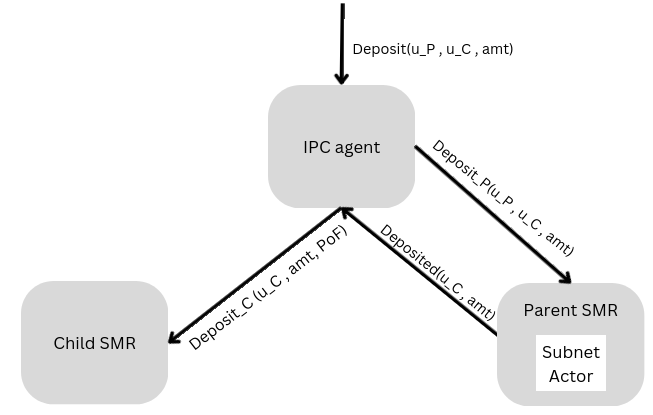
\includegraphics[width=\textwidth]{deposit}
     \caption{Events produced and consumed during a deposit.}
     \label{fig:deposit-old}
 \end{figure}
 
 \begin{figure}
     \centering
     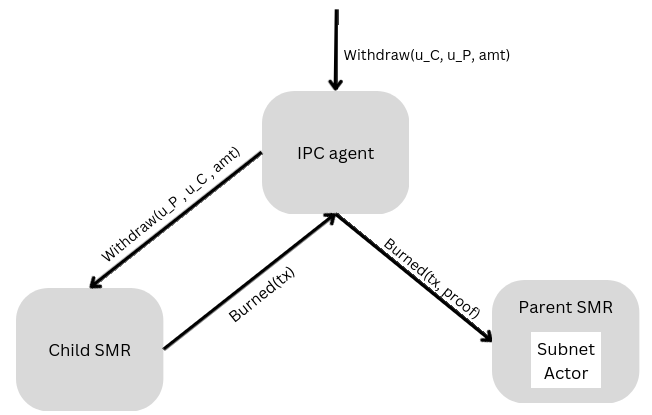
\includegraphics[width=\textwidth]{withdrawal}
     \caption{Events produced and consumed during a withdrawal.}
     \label{fig:withdrawal}
 \end{figure}
\noindent\textbf{Child Validator}\\
\textit{Deposits.} The child validator consumes an event \texttt{Deposited(TX)} produced by the IPC module upon which it updates its state in order to reflect this deposit. \\~\\
\textit{Withdrawals.} During operations that withdraw from child to parent subnets, the child validator first consumes a \texttt{WITHDRAW(TX)} from a user (or users) of the child subnet and then produces a \texttt{ChildWithdrawn(TX, [proof])} event to send to the IPC module. 
% The child validator does not yet terminate the withdrawal operation, as this may be aborted by the parent validator (if, for example, the withdrawal is invalid according to the state of the SA at the parent). The child validator eventually consumes a commit or an abort for each \texttt{ChildWithdrawn(TX, [proof])} that it produces. 
Depending on the type of subnet, the child validator can already provide a proof of global finality. If the child validator does not produce a proof of global finality then it is the job of the IPC module to produce such proof for the parent.\\~\\

\noindent\textbf{IPC Module}\\
\textit{Deposits.} The child validator first consumes a \texttt{ParentDeposited(TX)} transaction from the parent validator, and then performs the necessary operations to confirm the inclusion of the deposit into the child, depending on the type of deposit defined by the SA for this subnet and listed above in this document: on-chain voting, off-chain voting, local validity, etc. Once this deposit is confirmed by the IPC module, then the IPC module produces a \texttt{Deposited} event to be consumed by the child validator. The IPC module may also locally abort and not produce any events during deposits, should the deposit not be valid.\\~\\
\textit{Withdrawals.} During withdrawals, the IPC module first consumes a \texttt{ChildWithdrawn(TX, [proof])} event from the child validator, after which it produces a proof of the withdrawal that is valid for the SA at the parent (if the child subnet did not produce one already) and produces a \texttt{ChildWithdrawn(TX, proof)} to be consumed by the parent validator. 
% It is the responsibility of the IPC module to check the validity of the withdrawal given the state of the parent's SA, and to produce instead an \texttt{Abort} event to be consumed by the child validator if the SA's state is not consistent with the withdrawal. In the latter, it is possible that the IPC module finds proof of misbehaviour that should be reported, and in that case it also produces a \texttt{slash(...)} event to be consumed by parent, after which it will consume an event \texttt{Slashed(...)} from the parent validator and produce an event \texttt{Slashed(...)} to be consumed by the child validator.\\~\\
\noindent\textbf{Parent Validator}\\
\textit{Deposits.} The parent validator consumes a \texttt{Deposit(TX)} from a user (or users) and then produces a \texttt{ParentDeposited(TX)} event to be consumed by the IPC module.
\\~\\
\textit{Withdrawals.} During withdrawals, the Parent Validator consumes a \texttt{ChildWithdrawn(TX,proof)} event. 
% Then, it updates the current state of the SA, after which it produces a \texttt{Withdrawn(TX)} to be consumed by the IPC module. Alternatively, the parent might consume a \texttt{Slash(...)} event triggered by a withdrawal attempt, upon which it produces a \texttt{Slashed(...)}
\subsubsection{Other operations}
% \textit{Report/Slash.} There are two kinds of report operations: those that involve withdrawals, and those who are triggered at the child subnet but that should be reported at the parent. The former is already considered in the aforementioned flowchart for withdrawals, while the latter
We show reports in Figure~\ref{fig:report}. If the child validator detects provable misbehaviour, it notifies the IPC module through a \texttt{Report} event. Then, the IPC module follows the same path to request and notify slashing of the responsible deviants as the one showed for the withdrawal case.
\begin{figure}
     \centering
     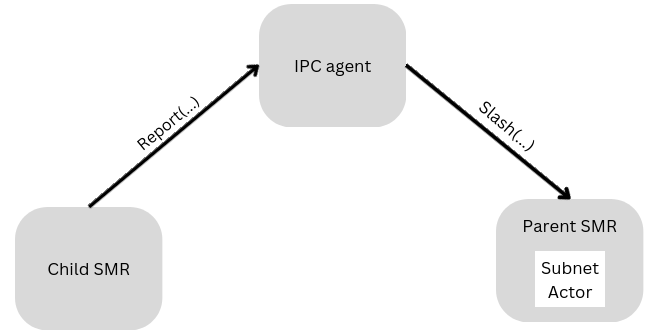
\includegraphics[width=\textwidth]{slash}
     \caption{Events produced and consumed during a report.}
     \label{fig:report}
 \end{figure}\\
 \textit{Checkpoints.} Checkpoints should follow the same procedure as withdrawals, except for: (i) the initial event that triggers the operation, as this is not necessarily a a transaction submitted by a user of the child subnet (most likely triggered by the IPC module); (ii) the payload of the events in the operation; and (iii) the local treatment of the events. The rationale for the events that are being triggered is analogous. 
 \arp{TODO: Propagate}
% \noindent \underline{IPC module interactions with the parent-validator:}%
% %\footnote{The interface is typically between two pieces of software on the same machine --- parent-node and child-node.}
% \begin{enumerate}
%     \item IPC-module queries the parent-validator if TX took effect in the parent (+ confidence parameter).
%     For example, the IPC-module observes (or is notified of) a relevant DEPOSIT transaction at the parent. 
%     \item IPC-module submits a transaction $TX$ to the parent-validator (the parent-SMR module). Examples:
%     \begin{itemize}
%         \item the IPC-module submits a WITHDRAW transaction $\langle TX(SA:g' \rightarrow^{+2} G, proof)\rangle_{Guy}$ to the parent-validator.
%         \item the IPC-module submits a CHECKPOINT transaction $\langle TX(SA:\textit{governance} \rightarrow^{+\textit{tip}} G, \textit{data}, \textit{proof})\rangle_{Guy}$ to the parent-validator.%
%         \footnote{Since~$G$ is the proposer and pays the transaction fee, the governance account ``reimburses"~$G$.}
%         \item the IPC-module submits a REPORT transaction to the parent-validator. \guy{TBD}
%     \end{itemize}
%     \item $getStateOf(SA)\rightarrow$ \guy{TBD}
    
% \end{enumerate}
% \vspace{2ex}

% \noindent \underline{Parent SMR invocations of $SA$ (the IPC smart contract):}
% \begin{enumerate}
%     \item \textbf{minimal interface} \texttt{DEPOSIT(subnet-account, amount)}\\
%     Example: \texttt{DEPOSIT($g'$, $2$)}\\
%     Increases a subnet client's balance by a given amount.
%     \item (\textbf{Including sanity check}) invoke DEPOSIT(Source, $SA:g$, amt). This enables the sanity check --- verify that Source (possibly restricted to $G$) has the funds to transfer.
%     \item \texttt{REPORT(violation, proof, reporter)} \guy{TBD}
%     \item apply \texttt{CHECKPOINT(data, proof)} \guy{TBD}\\
%     updates the data stored in $SA$ according to the new data in the checkpoint (e.g., updated account balances).
%     \item \texttt{Transfer(SA:governance$\rightarrow^{+\textit{amt}}G$, proof)} \guy{TBD}\\
%     Transfer money from the governance account to a specified account at the parent if $proof$ satisfy some condition. E.g., reimburse the proposer of a checkpoint.
% \end{enumerate}

% % \noindent \underline{IPC actor (smart contract) invocations of parent SMR:}
% % \begin{enumerate}
% %     \item \texttt{WITHDRAW(subnet-account, parent-account, amount)}\\
% %     Example: \texttt{WITHDRAW($SA:g'$, $G$, $2$)}\\
% %     Increases a parent client's balance by a given amount whilst reducing the child's account representation (the snapshot stored at SA in the parent) by the same amount.
% % \end{enumerate}

% \noindent \underline{IPC module interactions with the child-validator}

% \begin{enumerate}
%     \item $ProveGlobalFinality(tx) \rightarrow proof$: This function returns a proof that transaction $tx$ has been ordered and executed by the child SMR system and is final. This proof needs to be able to convince the SA (smart contract executed by the parent) of the $tx$'s finality. This is used for withdrawals: The SA only transfers the corresponding tokens to $G$ after verifying $proof$.
% \end{enumerate}

\subsection{additional points and future topics}
Non essential thing to think about in the future.
\begin{itemize}
    \item Entity observing parent replicated state and submitting corresponding transactions to the child SMR system (could be the user's laptop, a validator node, a third party, ...)
    \item finality function possibilities. E.g., varying according to amount, potentially slashed amount, network/faulty assumptions, etc. -> trade-off performance/security
    \item atomicity operations (atomic swap/atomic execution), IBC-like bridges 
    \item Alfonso: Fraud proofs and gas fees distribution. Two under-defined.
    \item Alfonso: if you don't mind including to your backlog of under-defined things: \url{https://github.com/consensus-shipyard/ipc-actors/issues/22} Also out of scope for M2, but really worth having for M3 and to answer future questions
\end{itemize}

 % - Intro
 %   - Overview
 % - Model
 % - Components and their Interfaces
 %   - Parent subnet node
 %   - Child subnet node
 %   - IPC module
 %   - Subnet actor
 % - IPC Functionality
 %  - Minimum required per subnet
 %    - Withdrawal/Deposits Interfaces
 %    - Other Operations? (Propagate?)
 %  - Enhancements
 %    - Checkpointing interfaces
 %    - Propagate
 %    - Reporting/Slashing interfaces
 %    - Atomic execution/swap, IBC-like bridges
 %  - Future stuff (google docs?)
 %    - Withdrawal at ancestor (skip parent(s)) (with timeout) etc.
 % - Implementations/templates
 %  - Different types and trade-offs of checkpoint triggers 
 %    - Periodically: time, #blocks, #withdrawn, etc.
 %    - At request: (this one is not governance funded)
 %    - Combinations of these 
 %    - Slashing functions
 %    - Atomic execution types?
 
